\subsection{Satisfiability Solvers}
A SAT solver basically tries to find a solution, an assignment of all variables so that the formula is true, to a specified boolean formula. All modern SAT Solvers additionally return a specific assignment if possible or otherwise specify that the formula is not satisfiable.

As an example take the following formula as an input $A \land \lnot B$ there's only one variable assignment where the formula evaluates to true, namely A = true and B = false.

An unsatisfiable example would be the following formula: $A \land \lnot B \land (\lnot A \lor B)$.  There's no possibility how to assign boolean values to A and B so that the formula evaluates to true as shown by table \ref{table:unsat_truth_table}, therefore its unsatifable.
\begin{table}[!htbp]
\begin{adjustbox}{width=\columnwidth}
\begin{tabular}{ |c|c|c|c|c| } 
 \hline
 $A$ & $B$ & $\lnot B$ & $\lnot A \lor B$ & $A \land \lnot B \land (\lnot A \lor B)$ \\ 
 \hline
 True & True & \highlight{False} & True & False \\ 
 True & False & True & \highlight{False} & False\\ 
 \highlight{False} & True & \highlight{False} & True & False\\ 
 \highlight{False} & False & True & True & False\\ 

 \hline
\end{tabular}
\end{adjustbox}
\caption{Truth table for the unsatisfiable example. The partial expressions that lead to the expression evaluating to false are highlighted.}
\label{table:unsat_truth_table}
\end{table}

To simplify the task, the formula has to meet certain criteria to be allowed as an input to a SAT solver. The most important criteria is that the formula has to be in the conjunctive normal form, hereinafter referred to as CNF. 

In the following paragraph, the rules of CNF will be explained followed by some examples. The next paragraph shows that this restriction to CNF is not a big problem, because it's possible to transform any boolean formula into CNF\cite{Jackson:2004:CFC:2103144.2103160}.
\subsubsection{CNF}
CNF uses variables like $A$ or $B$ which can either be true or false.
These variables are used in literals. Each literal consists of exactly one variable or its negation. It's allowed to use a variable in multiple literals, but only one of the values \{true, false\} can be assigned to a variable, which will be used in the whole formula.

Consider the two example literals: $A$ and $\lnot B$

These literals can be combined to form a clause. Each of the clauses consists of any number of literals that are in a disjunctive relation. 

Let's suppose the following three clauses: 
$$A \lor B$$
$$B \lor \lnot C$$ 
$$C$$
Each formula in CNF consists of any number of clauses which are in an conjuctive relation. For example: $$clauseOne \land clauseTwo \land clauseThree$$\\
The whole boolean formula would therefore be: $$\underbrace{(A \lor B)}_{clauseOne} \land \underbrace{(B \lor \lnot C)}_{clauseTwo} \land \underbrace{(C)}_{clauseThree}$$\\

If a boolean formula is not in the CNF it's necessary to convert it before entering into the SAT solver. For example the boolean formula $\lnot(A \lor B) \lor C$ can be converted into ($\lnot A \lor C) \land (\lnot B \lor C)$

There are different kinds of special clauses:
\begin{itemize}
\item empty clause
\item unit clause
\item binary clause
\end{itemize}
The empty clause contains no literal and is in literature denoted with different symbols. In this publication, an uppercase lambda $\Lambda$ will be used as suggested by Gomes et al \cite{Gomes2008SatisfiabilityS}.
The empty clause always evaluates to false, because there is no possibility to assign a variable which lets the clause evaluate to true.

The unit clause contains exactly one literal. This literal either contains a variable or its negation as described before. 
The clauses $A$ and $\lnot A$ are both unit clauses. 
The unit clause is a special case because its possible to deduce the value of the variable used in the unit clause.
If a CNF formula should evaluate to true and contains a unit clause the unit clause must also evaluate to true. 
This property will be heavily used by the SAT solver.

Consider the example clauses used above. In clause $A$ the variable $A$ has to be true and in the other example, $\lnot A$ the variable $A$ has to be false.

The binary clause contains exactly two literals. At a first glance, this does not look very special at all, but binary clauses allow powerful optimizations. As soon as one of the two variables gets assigned it's possible to deduct the value of the other variable. This, for example, allows it to efficiently track the event when a variable can be deducted.
\subsubsection{DPLL}

There are many different methods how a SAT Formula can be solved. The most simplistic approach would be to just brute-force the formula and try to evaluate the formula for every possible combination of variables. This works well for a small number of variables but does not scale, because the computation time increases exponentially. In this chapter, the method of the DPLL procedure will be presented. It is the basis for many of the currently used algorithms and fortunately not too hard to understand.

The predecessor of this method was first presented in 1960 by Davis and Putnam \cite{Davis:1960:CPQ:321033.321034} and improved in 1962 by Davis, Logemann and Loveland \cite{Davis:1962:MPT:368273.368557}, hence the name DPLL which consists of the initials of the inventors.

Even though the worst case still requires exponential time, normally these algorithms provide massive computational benefits. In this publication, the recursive version of the algorithm will be used because it's much easier to understand some of the key ideas. Note that the algorithm also exists in iterative versions, which are able to reduce the memory usage \cite{Gomes2008SatisfiabilityS}.

The algorithm will be represented by two parts of pseudo-code algorithms \ref{algDPLLRecursive}, \ref{algUnitProgagate}.

The algorithm DPLLRecursive shows the general structure of the approach, but the algorithm UnitPropagate actually is similarly important.

\begin{algorithm}[caption={DPLLRecursive}, label={algDPLLRecursive}]
 input: $F$: boolean formula in CNF-Form
	$\rho$: assignment of variables
 output: assignment that satisfies F or 
	UNSAT if no assignment is possible
 begin
   $(F, \rho)$  $\gets$ UnitPropagate
   if $\Lambda \in F$
       return UNSAT
   if $F = \emptyset$
       return $\rho$
   $l \gets$ a literal not assigned by $\rho$
   $result \gets$ DPLLRecursive($F \cup \{l\}, \rho$)
   if $result \neq UNSAT$
       return result
   return DPLLRecursive($F \cup \{\lnot l\}, \rho$)
\end{algorithm}


\begin{algorithm}[caption={UnitPropagate}, label={algUnitProgagate}]
 input: $F$: boolean formula in CNF-Form
	$\rho$: assignment of variables
 output: $F$: updated boolean formula
	$\rho$:updated assignment of variables
 begin
   while $F$ contains no empty Clause
   and there exists a UnitClause $xClause$
       $xLiteral \gets$ the only literal of $xClause$
       while there exists an $yClause$ in $F$
       which contains an $xLiteral$
           $F \gets F \setminus \{yClause\}$     
       while there exists an $zClause$ in $F$
       which contains an $\lnot xLiteral$
           $newZClause \gets zClause \setminus \{\lnot xLiteral\}$
           $F \gets (F \setminus \{zClause\}) \cup \{newZClause\}$
       $\rho \gets \rho \cup \{xLiteral\}$
   return $(F, \rho)$
 end
\end{algorithm}


First, the unit propagation is executed, after that it's checked if either of the base cases is reached. 
There are only two base cases. Either the formula contains no more clauses that result in a satisfying formula (as shown in lines 9-10) or the formula contains an empty clause that results in UNSAT (as shown in lines 7-8).

The next step (line 11), also called branching step, selects the literal $l$, which should be eliminated in the next recursion.

The last step of the DPLLRecursive is to call itself twice with new input. In one case a new unit clause with the selected literal $l$ is added to the formula (line 12), in the other case the unit clause with the negation of the literal, $\lnot l$, is added (line 15).

\begin{figure}
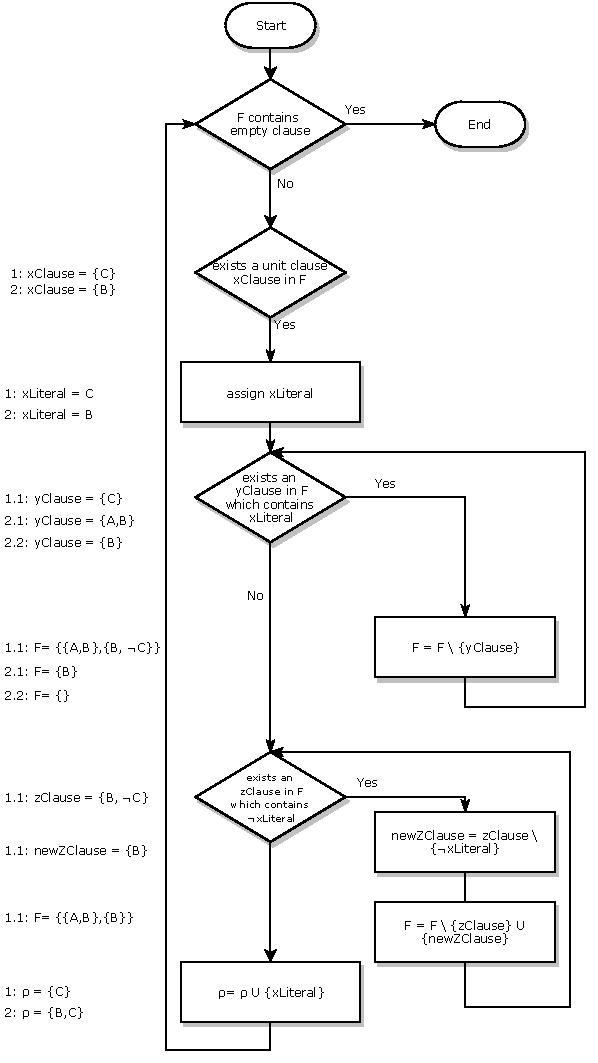
\includegraphics[width=\columnwidth]{unitpropagate}
\centering
\caption{Flowchart of the unit propagate algorithm as desribed in algorithm \ref{algUnitProgagate}.\\ Annotated with the actual values that are assigned for the input $F=(A \lor B ) \land (B \lor \lnot C) \land (C)$ and $\rho = \{\}$. The number on the left side is representing the current iteration.}
\label{fig:unitpropagate}
\end{figure}

The step where the first recursion ends in UNSAT and returns to the base is called backtracking. In the recursive version, this is very simple because there's literally nothing to be done. However in the iterative version, that is used in practice, backtracking can be very sophisticated.

The second part of the algorithm, called UnitPropagate, which is the first step of the DPLL algorithm, will try to assign values to all variables, which can be deducted.

The easiest way to determine the value of a variable is if there is any unit clause in the formula. Because CNF defines that every clause has to be true by itself, the clause and the literal have to be true as well.

Consider the following example: Suppose the unit clause $A$ which is part of the formula, the value true can be assigned to the variable A. On the other hand, suppose the unit clause $(\lnot A)$, the value false can be assigned to the variable A.

After a specific value was assigned to the variable the formula can be updated to reflect the changes. 

As a first step, all clauses that contain the same literal (lines 8-9) have to be removed, as these clauses automatically evaluate to true. 

The second step is to remove all occurrences of the negated literal from all clauses (lines 10-11). This step is possible because the negated literal will always evaluate to false and an $\lor false$ combination is redundant.

This reduction can result in new unit clauses, which then will be propagated until no more feasible clauses can be found or an empty clause $\Lambda$, which leads to an unfeasible formula, is constructed.



\subsubsection{Improvements of today's SAT solvers}
The key differences between the original DPLL Algorithm and currently developed SAT solvers lie in the improvement of either the branching selection of the literal, the backtracking after a branch ends in an UNSAT state and some improvements to the unit propagation.
\todo{Some more details}